\documentclass[12pt]{article}
\usepackage[margin=1in]{geometry}
\usepackage[pdftex]{graphicx}
\usepackage{multirow}
\usepackage{setspace}
\usepackage{enumitem}
\pagestyle{plain}

\begin{document}

\noindent
% Course information
\begin{tabular*}{\textwidth}{l @{\extracolsep{\fill}} r}
  & \multirow{3}{*}{
\includegraphics[height=1.0in]{logo.jpg}} \\
  \large Quantum Mechanics & \\
  \large Fall Quarter 2023 & \\
  \large Physics 115A & \\
\end{tabular*}
\vspace{10mm}

\noindent
% Professor information
\begin{tabular}{ l l }
  \multirow{6}{*}{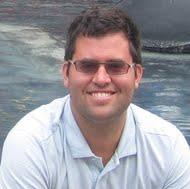
\includegraphics[height=1.25in]{mike.jpg}} & \\
  & \\
  & Michael Mulhearn \\
  & mulhearn@physics.ucdavis.edu \\
  & Physics 317 \\
  & \\
\end{tabular}
\vskip 0.5cm

\noindent
\begin{tabbing}
\hspace*{8em} \= \kill 
\textbf {Lectures:} \> M,W,F 9:00-9:50 AM in Roessler 55 
\end{tabbing}
\noindent
\begin{tabbing}
\hspace*{8em} \= \kill 
\textbf{Textbook:} \> Intro. to Quantum Mechanics (3rd Ed.) by Griffiths and Schroeter \\
\> Lecture notes will be available on course website.
\end{tabbing}
\noindent
\begin{tabbing}
\hspace*{8em}\= \hspace*{14em} \= \kill 
\textbf{Course TAs:} \> Ben Eustis-Guthrie \> (bmguthrie@ucdavis.edu) \\
                     \> Umut Oktem \> (ucoktem@ucdavis.edu) 
\end{tabbing}
\noindent
\begin{tabbing}
\hspace*{8em}\= \hspace*{14em} \= \kill 
\textbf{Office Hours:}    \> Mulhearn: \> TBA \\
    \> Problem Solving Session: \> TBA \\
    \> Eustis-Guthrie: \> TBA \\
    \> Oktem: \> TBA \\
\end{tabbing}
\noindent
\begin{tabbing}
\hspace*{12em}\= \kill 
\textbf{Midterm Exam:} \> 1.1-1.6,2-2.4 Date TBD (Aim for Nov 8)\\
\textbf{Final Exam:} \> Wed, December, 13 2023 6:00 PM in Roessler 55
\end{tabbing}
\noindent
\textbf {Course Description:}\\
Introduction to quantum mechanics.  We will introduct the
Schr\"odinger Equation and it's probabilistic interpretation.  We will
then hone our understanding and intuition with a series of examples:
infite wells, harmonic oscillators, free particles, finite wells,
delta function potentials, and the WKB approximation.  Grounded by
these examples, we will formalize our understanding of quantum
mechanics with Hilberth Space, Observables, Uncertainty Principle, and
introduce the powerful Dirac Notation.\\ 

\newpage
\noindent

\noindent
\textbf{Homework:}\\
Homework and due dates will be posted on the course website.  The best way to prepare for the exams is to solve problems yourself or by actively participating within a study group.  Do not post homework problems to internet forums or use solutions found online.  Always do you own work and be prepared to explain it.\\

\noindent
\textbf{Cheating:}\\
Cheating is in the long run counterproductive, but I can understand that it is frustrating when it seems the cheaters are getting away with it in the short term.  Therefore, this class will include some countermeasures against cheating.  Most homework assignments will include practice problems which are graded by effort only.  Anyone cheating on these problems would be risking getting caught for no benefit to their grade.  For newly written problems, we will be monitoring the cheating websites to see if they begin to appear.  If they do, we may implement additional countermeasures: such as looking for tells in the online solutions, or starting weekly homework quizzes, just to mention a few.
The best safeguard against cheating is the midterm and final exam.  If you do all your homework yourself, you should be well prepared for those exams.

\noindent
\textbf {Grades:}\\
Final grades will be approximately $60\%$ Homework, $20\%$ Midterm Exam, and
$20\%$ Final Exam.  Your worst homework score will be dropped.\\
\noindent

\noindent
\textbf {Course Schedule}:\\
Here is the anticipated schedule for the course.  It may change as the
course progresses.  Attendance on Nov 22 (the day before Thanksgiving) will be worthwhile but optional.
The pace will be about one section per lecture: brisk but doable.  Please keep up with the reading even if the lectures fall behind.\\

\noindent
\textbf {Lectures}:\\

\noindent
\begin{tabular}{llll}
\textbf{Week} & \textbf{Dates} & \textbf{Topics} & \textbf{Reading} \\
\hline
1  & Sep 27,29         & Wave Function, Schrondinger Equation & 1.1-1.4, P1.14 \\
   &                   & Momentum Operator  & 1.5 \\
\hline
2  & Oct 2,4,6         & Uncertainty Principle & 1.6, P1.7 \\
   &                   & Stationary States, Infinite Square Well & 2.1, 2.2 \\
   &                   & Fourier Series   & \\
\hline
3  & Oct 9,11,13       & Harmonic Oscillator & 2.3 \\
   &                   & Free Particle, Momentum Space & 2.4 \\
   &                   & Fourier Transform  &  \\
\hline
4  & Oct 16,18,20      & Delta Function Potential & 2.5 \\
   &                   & Finite Square Well & 2.6, P2.52\\
   &                   & WKB Approximation & 9.1,9.2 \\
\hline
5  & Oct 30, Nov 1,3   & Hilbert Space, Observables, Operators & 3.1, 3.2, 3.3\\
\hline
6  & Nov 6,8           & Catch-up and Midterm Nov 8 (tentative) \\
\hline
7  & Nov 13,15,17      & TBD (Chap 3) \\
8  & Nov 20,(22)       & TBD (Chap 3) \\
9  & Nov 27, 29, Dec 1 & TBD \\
10 & Dec 4,6,8         & TBD \\
\hline
\end{tabular}\\ \vskip 1cm

\end{document}

